
\section*{Abstract}
The main goal of this project is to explore and examine the properties of the 802.11 specification. Wireless communication/security is critical to maintaining the internet infrastructure and therefore a focus of both hackers and network administrators. As data is sent over a shared medium it is possible with passive scanning to obtain traffic and analyze it. By doing so, two advanced attacks have been examined. Deauthentication attacks have been exploited in order to deny service for clients(DoS) on the WLAN, whilst WEP secret key cracking has been used to obtain clear text traffic. WEP was one of the first ways to encrypt wireless data, but has glaring flaws in its algorithm. It's been possible to crack the password for a network secured by WEP and shown that by capturing packets from a single user on an AP, all data that has been sent over the medium can been decrypted. The WLAN has been mapped by a written WiFi-scanner in Scapy (Python library) in connection with our deauthentication attacks that show key information on the WLAN. A deauthentication attack has been successfully completed on a modern device after identifying it with our WiFi-scanner. This shows that even secure networks using technologies in use today, are still at risk of certain attacks.

\newpage
\tableofcontents
\newpage

\section{Contributers}

\begin{table}[!htbp]
\centering
\begin{tabular}{|l|l|l|}
\hline

\textbf{Section}   & \textbf{Contributer} & \textbf{Reviewer} \\ \hline
Abstract           & Oliver               & Lucas             \\ \hline
Introduction       & Nicklas              & Oliver            \\ \hline
Functionality      & Everyone             & Everyone          \\ \hline
Theory 4.1         & Lucas                & Oliver            \\ \hline
Theory 4.2         & Nicklas              & Oliver            \\ \hline
Implementation 5.1 & Oliver               & Nicklas           \\ \hline
Implementation 5.2 & Nicklas              & Lucas             \\ \hline
Implementation 5.3 & Lucas                & Oliver            \\ \hline
Tests 6.1          & Oliver               & Lucas             \\ \hline
Tests 6.2          & Nicklas              & Lucas             \\ \hline
Tests 6.3          & Lucas                & Nicklas           \\ \hline
Main Challenges    & Oliver               & Nicklas           \\ \hline
Timeplan           & Lucas                & Oliver            \\ \hline
Conclusion         & Nicklas              & Oliver            \\ \hline
\end{tabular}
\end{table}

\section{Introduction}
Wireless security has become increasingly critical due to the rapidly expanding use and need for internet access. Many devices use WiFi to connect to the internet, such as smartphones and laptops. As data over WiFi is sent via radio waves, thus using a shared medium there is a coherent risk when communicating. The data is at risk of being captured by bad actors and is prone to manipulation. Thus a need for strong encryption and control of said data is necessary. However, some security measures for wireless networks, still have vulnerabilities to exploit. One such attack, which is the focus of this report, is a denial-of-service (DoS) attack: the deauthentication attack. It's an attack where a user will be denied access to the network and thereby either disrupt a workplace or pave the way for other more sophisticated attacks such as the Evil Twin Attack\footnote{An Evil Twin attack is when the adversary creates an AP identical to the victim's, and then either forcing or tricking the victim's devices to connect to the malicious AP, thus obtaining a Man-in-the-Middle state.}.

This project will explore the theory and practical applications of deauthentication attacks on networks. Further, password cracking will be explored for secret keys used in the encryption of wireless network traffic using the now outdated WEP protocol. To achieve these goals, information about the wireless local area network (WLAN) has to be known. Thus, another goal for the project is obtain information of available SSIDs, clients connected, signal strength and so on.

When this project is done, the hope is to have explored the the theory and practical applications of deauthentication attacks on networks and the building blocks that make up data-packets in a wireless network. It is important to note that this project is for educational purposes only and should not be used for malicious activities.

\section{Functionality}
Our project constists of the following functionalities:
\begin{enumerate}
    \item Scan the WLAN and identify key information about clients/Access Points.
    \item Perform deauthentication attack on WiFi devices.
    \item Capture packets and obtain clear text by cracking password of WEP encryption.
\end{enumerate}

These functionalities are the core of the project. Wherein scanning and mapping the WLAN, is of a great importance. As this is nessecary for performing both deauthentication and password cracking. 

A typical user roadmap utilizing the scanning of the network in order to deauthenticate the user is shown on figure \ref{user-roadmap}.

\begin{figure}[!htbp]
    \centering
    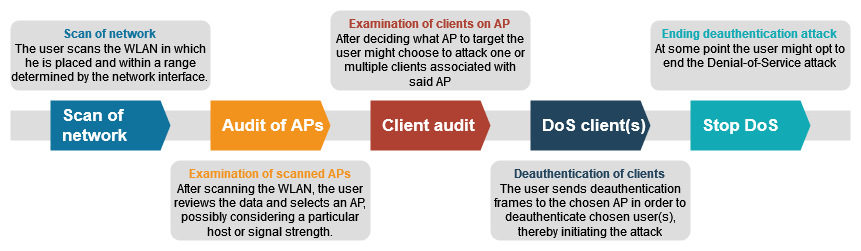
\includegraphics[width=0.9\textwidth]{Latex-Files/Billeder/Flowcharts/user-roadmap.png}
    \caption{A typical user roadmap}
    \label{user-roadmap}
\end{figure}

A deauthentication attack is a type of Denial-of-Service (DoS) attack that targets communication between a user and a WiFi access point \cite{Deauth}. It exploits a feature of IEEE 802.11 wireless networks that allows devices to disconnect from a network by the deauthentication management frame \cite{Deauth_Wiki}.
A deauthentication frame tells a device to stop communicating with the AP. It can be sent by either the AP or the device itself. It's normally used for legitimate purposes, such as ending a connection or switching to another network (handover); Yet there is no identification check performed in this procedure. Therefore an attacker can exploit this feature and send deauthentication frames to the AP with a spoofed\footnote{Spoofed: An illegitimate address to trick the victim.} client source address. This causes the connection to close making the spoofed device's connection end and probably reconnect. This exploitation has multiple use-cases. If done repeatedly or to multiple devices, this can disrupt or disable the network entirely, thus resulting in a DoS Attack. Meanwhile it can also be used to obtain an EAPOL 4-way-handshake for WPA or as a way to misguide a client to a rogue access point created by a malicious user to obtain a Man-In-The-Middle state, known as an Evil Twin Attack. 

The last point is password cracking. The product should be able to crack/obtain the WiFi-password in the WEP algorithm. WEP is one of the most basic WiFi algorithms. It is an outdated and non-secure algorithm and the product utilizes Aircrack-ng's PTW method to recreate the passwords on the APs \cite{aircrack-ng}. The method needs data-packets from users on the network containing initialization vectors and those are captured by the WiFi scanner, as that is it's primary functionality. When the scanner has obtained enough packets, around 10.000, the password cracker should then be able to obtain the passwords using Aircrack-ng. This part utilizes a tool that is already known, thus a greater focus here will be largely theoretical.

The implementations are mainly based on the python library Scapy \cite{scapy} to implement the functionalities. As our network interface has to be put in monitor mode a UNIX environment is used. The long-term goal is to use a raspberry pi later, to obtain mobility and a uniform platform. 
The network interface is a Realtek DWA 131-E1 dongle, as it is cheap and allows for the usage of monitor mode. The UNIX platform has the consequence of limiting the use of the implementation to a specific operating system. Though this should be able to be ported to Windows and MacOs if need be. Here the Linux-sub-system (WSL) on Windows might be exploited \cite{WSL_exploit}.
The positive side of using UNIX is that we can implement the program on many types of systems as we use a virtual machine to create the product. Thus making conversion to a raspberry pi easier. The negative side is that we have to use a virtual machine which can create problems with drivers and performance. 

\subsection{Mapping of networks}
This block takes the physical data being sent in the wireless space, and transforms it into information that the other blocks need and use. It contains a table that holds the information as sub-blocks, for instance access points in the WLAN, the signal strength of the AP and which channels are used as well as the clients on said AP. This mapping can be done via beacon management frames used by APs to announce their respective presence. Likewise probe management frames can be used to understand what APs a client has been associated with in the past.
The block also contains a way of collecting data-packets containing initialization vectors and sending them to the password cracking block. 

\newpage
\subsection{Deauthentication}
This block handles deauthentication, wherein we deny clients access of certain APs or all wireless internet usage. Thus making the sub-blocks: 
\begin{itemize}
    \item Client
    \item AP
    \item Channel
\end{itemize}


\subsection{Password cracking}
This block handles the actual cracking of WEP from data-packets collected from the mapping block. The data should be combined into a single file which can then be analysed and the password/passkey found.

\section{Theory}

SKRIV NOGET OM SCAPY

The primary conceptual framework underpinning this project revolves around the 802.11 standard \cite{IEEE802.11}. The 802.11 standard is a set of wireless network protocols developed by the Institute of Electrical and Electronics Engineers (IEEE). The first version of the standard, 802.11, was released in 1997, and since then, several revisions and amendments have been made to improve the technology and increase its capabilities \cite{ETHW}.

The 802.11 standard uses radio waves to transmit data between devices within a WLAN without the need for cables or wires. This makes it a popular choice for connecting mobile devices to the internet, especially in homes, offices, and public places such as cafes, airports, and hotels \cite{Public_WiFi}.

Throughout the project, programming will be done mainly in python, using the library Scapy for sniffing, analyzing and transmitting packets. Scapy is a program written in Python, that gives the ability to construct, decrypt, send, capture packets and much more \cite{IEEE_Scapy}. 
Scapy gives us tools for analyzing 802.11 frames, thus providing the information contained in 802.11 frames. Packets in Scapy are created as objects with layers built on top of each other to define the type of the packet. 
\\

\begin{figure}[!htbp]
    \centering
    \includegraphics[width=0.5\textwidth]{Latex-Files/Billeder/WiFi_Types.png}
    \caption{WiFi types and Subtypes}
    \label{WiFi Types}
\end{figure}

There are three frame types in 802.11: management frames, control frames, and data frames.\cite{Amit802.11frames, DefinitiveGast}. Figure \ref{WiFi Types} shows some of the types and subtypes of different frames with a focus on management frames, since that is what our project is focused on.  Management frames are used by APs to join and leave the basic service set (BSS). They have a MAC header, a frame body, and a trailer. These frames are needed because it is difficult to connect to a wireless network compared to a wired network. With a wireless connection, all data is sent everywhere and each router and user needs to know which data-packets to ignore and which to receive. This is done via management frames where a user associates with an Access Point (AP) and agree on conditions, such as security and speed. For a user to know which APs are near, it needs to scan the surrounding area. This is done via 2 ways of scanning: Active scanning and passive scanning.

In passive scanning each AP broadcasts beacon frames and a user sends an association request to the AP it wants to connect to. In active scanning the user broadcasts probe requests and each AP responds to this request with a response back to the user. When the user then wants to connect to an AP that has responded it sends an association request to that specific AP. 

\subsection{WEP \& WiFi security standards}
Wireless networks also need security while sending packets, i.e. integrety and confidentiality. To ensure confidentiality, data-frames are encrypted with some sort of security standard. The oldest widespread type being Wired Equivalent Privacy (WEP). It had major security flaws that allowed hackers to bypass the algorithm and read the data being sent\cite{WEP1}. Therefore a new protocol for network security was in need. WiFi Protected Access (WPA) was soon after developed and implemented from 2003 and onwards\cite{WEP3}. 

WEP uses a secret key to encrypt packets sent between a client and the AP \cite{WEP2}. Although, a fundemental underlying problem with WEP is, that WEP uses the RC4 encryption algorithm, which is known as a stream cipher. A stream cipher operates by making a short key into an infinite random key-stream. The client uses the XOR operator on the key-stream with the plain data to produce the encrypted data. The AP has a copy of the same used key, and uses it to generate an identical key-stream. The AP then performs the XOR operation on the key-stream with the encrypted data thus obtaining the exact same plain data back. This type of encryption is easy to misuse, since by flipping a single bit in the encrypted data, the plain data will also have a corresponding single bit flipped. Furthermore the XOR'ed data can be found via statistical analysis of key-streams thereby recovering the plain data.

\begin{figure}[!htbp]
    \centering
    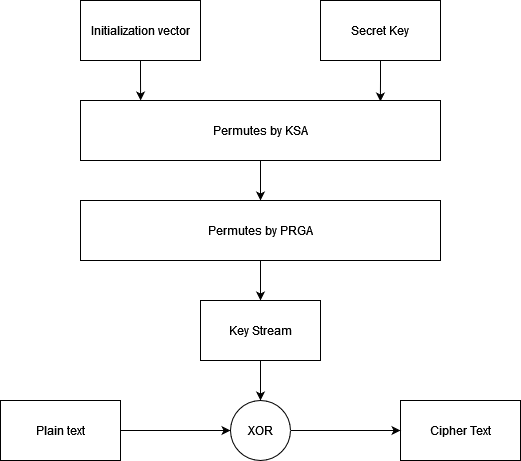
\includegraphics[width=0.4\textwidth]{Latex-Files/Billeder/RC4.png}
    \caption{Simplified RC4 algorithm \cite{geeks}}
    \label{RC4}
\end{figure}


WEP has incorporated defenses against these 2 types of attacks, but they are implemented poorly. The defense against flipping bits is integrity checks in the packet, implemented as a CRC-32 checksum. Unfortunately this is linear, which means that it is possible to find the difference between 2 CRC's because the bits that are flipped in the encrypted data is deterministic and therefore an attacker can adjust the checksum and then it is believed that the integrity of the packet is kept, when in reality it isn't.

The defense against the statistical attack is an initialization vector to decrease the chance of reuse of key-streams. The vector is only a 24 bit field and that guarantees the reuse of key-streams because the vector is only made up 24 bits and when thousands or millions of data-packets are sent, reuse will happen often. It would take around 110.000 data-packets to ensure reuse \cite{Random_map}. Because of this, the attacker can easily pick up enough data to perform statistical analysis of packets using the same key-stream and then recover the plain data.

Fortunately mitigation for the flaws of WEP have become industry standard since the WPA2 protocol, which was a development of the intermediate measure WPA as a security update to fix many of WEP's problems \cite{WPA2_1}\cite{WEP3}. It was released in 2004 in the 802.11i amendment to the original 802.11. WPA2 uses CCMP protocol which is a development of the AES security algorithm. It rids the network encryption of the previously mentioned security vulnerabilities. 

\subsection{Deauthentication in WLAN}
The authentication of clients and APs can be exploited by deauthentication attacks. The theory behind this attack is based on the 802.11 standard, which allows clients to disconnect from an AP using a deauthentication frame\cite{IEEE802.11}.

Deauthentication frames are frames of the management type as seen in figure \ref{WiFi Types}, and have the overall structure as such. Therefore the deauthentication frame contains, among other things, 3 addresses. These addresses being the destination address, the source address, and the BSSID of the AP's wirelsess interface, the address of the AP  These three addresses are what can be altered in order to perform a deauthentication attack. One of the fields in a deauthentication frame is the reason code, which is 16-bit. This defines the reason for the termination of the connection. There can thus be upwards of 65535 reason codes, yet only about 66 is utilized \cite{Cisco_Deathentication_reasoncodes}. Apart from a reason code, the frame body includes vendor specific elements, and the Management MIC IE(MMIE) \cite{IEEE_802.11w}. Though this is not always present. 

In a deauthentication attack, an attacker sends a series of forged/spoofed deauthentication packets to the target client or AP, pretending to be the legitimate access point or client. This causes the target to disconnect from the network and require reauthentication, disrupting the communication between the client and the access point.

802.11w, released in 2009, introduces protected management frames thereby combatting attacks such as deauthentication attacks. This is achieved by ensuring the integrity in the management frame. The integrity check is achieved by the sender calculating a Message Integrity Check (MIC) value, and appending this to the frame. The receiver then calculates the MIC value using the same algorithm, and compares the two. If the two MIC values match, the frame is considered to not having been tampered with, and thus marking it as authentic. Furthermore a frame sequence number(FSN) is introduced, which is used to prevent replay attacks. Replay attacks are not something we will be covering in this project and therefore it wont be analyzed in this report. 
The MMIE is thus only in use when protected management frames are enabled \cite{IEEE_802.11w}. Protected management frames were introduced in order to combat the deauthentication attack. Since the deauthentication frames without protected management frames has no integrity check by nature, this creates a sizeable vulnerability for a network as attacks such as the deauthentication attack can be exploited.

\section{Implementation}

The implementation is based purely on Python3 and the library Scapy. Figure \ref{802.11 Security} shows a UML-class-diagram of the two classes utilized in the implementation (without CLI). The Scanner class can hold multiple WiFi objects. The Scanner class can be seen as the main class holding and performing the core functionalities. For now there are some functions that may be bloated in conjunction with a possibility of simplifying the classes. As this is one of the first iterations of the code this is to be expected. 

\begin{figure}[!htbp]
    \centering
    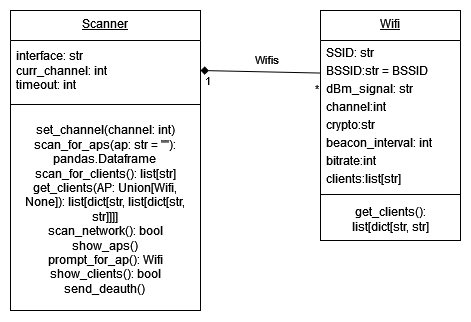
\includegraphics[width=0.5\textwidth]{Latex-Files/Billeder/Flowcharts/uml_diagram.png}
    \caption{UML diagram of Scanner and WiFi classes}
    \label{802.11 Security}
\end{figure}

\subsection{Mapping of networks}
The WiFi-scanner is the backbone of our implementation. It listens to all data that is transferred over WiFi and subsequently creates the lists that the deauthentication uses and captures packets for the password cracker. The point of this functionality is to gather information about APs and the associated clients, the logic for this implementation is showed in figure \ref{Flowchart} as a flowchart.

Firstly a system check is performed to ensure that the program is running on a UNIX system, as the program is not compatible with other systems. A possible operating system error is shown on figure \ref{W_error}

\begin{figure}[!htbp]
    \centering
    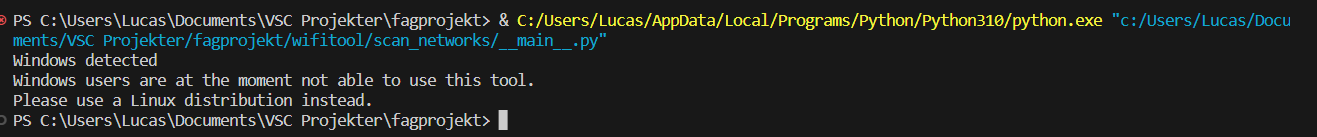
\includegraphics[width=0.5\textwidth]{Latex-Files/Billeder/Implementation/Windows_error.png}
    \caption{Windows error}
    \label{W_error}
\end{figure}

Then the program checks if the user is running the program as root, as this is required for the program to function properly. The passive scan is split into two main tasks, the first being the scanning for APs and the second being the scanning for clients. 
A possible optimization of the program could be combining these two tasks into one, however this would require a more complex implementation, and would not be as readable.
The scanning for APs is done by sniffing for beacon frames, which are sent by APs to announce their presence.
The sniffing is done by using the Scapy function "sniff", which takes a filter as an argument, this function is used when scanning for APs. The filter "type mgt, subtybe beacon" is applied in order to only sniff for beacon frames when looking for APs, and the function is set to run for a specified timeout duration. This is done to ensure that the program does not run indefinitely, and thereby potentially causing issues with the system. The code for part of this is shown in figure \ref{Scan1}.

\begin{figure}[!htbp]
    \centering
    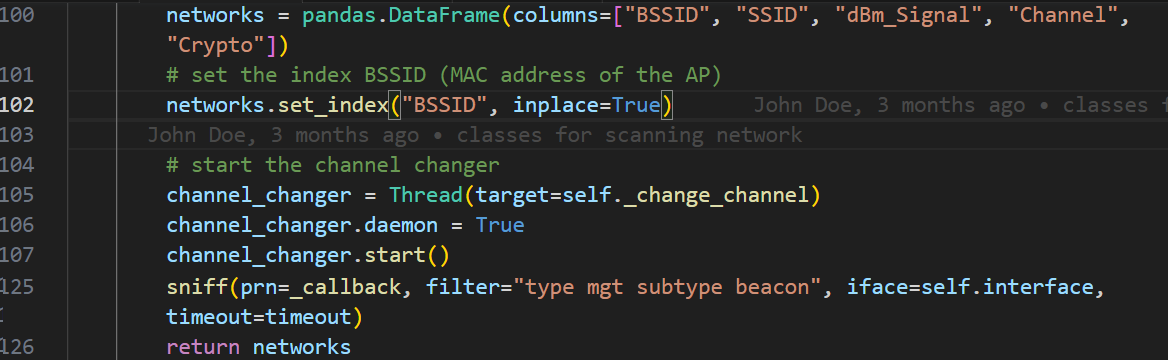
\includegraphics[width=0.45\textwidth]{Latex-Files/Billeder/Implementation/AP_Scan.png}
    \caption{Code for the sniffing with Scapy}
    \label{Scan1}
\end{figure}

The scanning is done on each network channel in turn, where it scans for beacon frames from the APs. It returns the BSSID (MAC-address), SSID, signal strength, channel and the cryptography of each AP.

To obtain information about clients we use the APs that we found and then look at packets being sent and check if the packet is sent from a client. This is then returned with the code shown in figure \ref{Scan2}. We can see that \lstinline{WiFi.get_clients()} is the code that gets the clients for each AP.
\begin{figure}[!htbp]
    \centering
    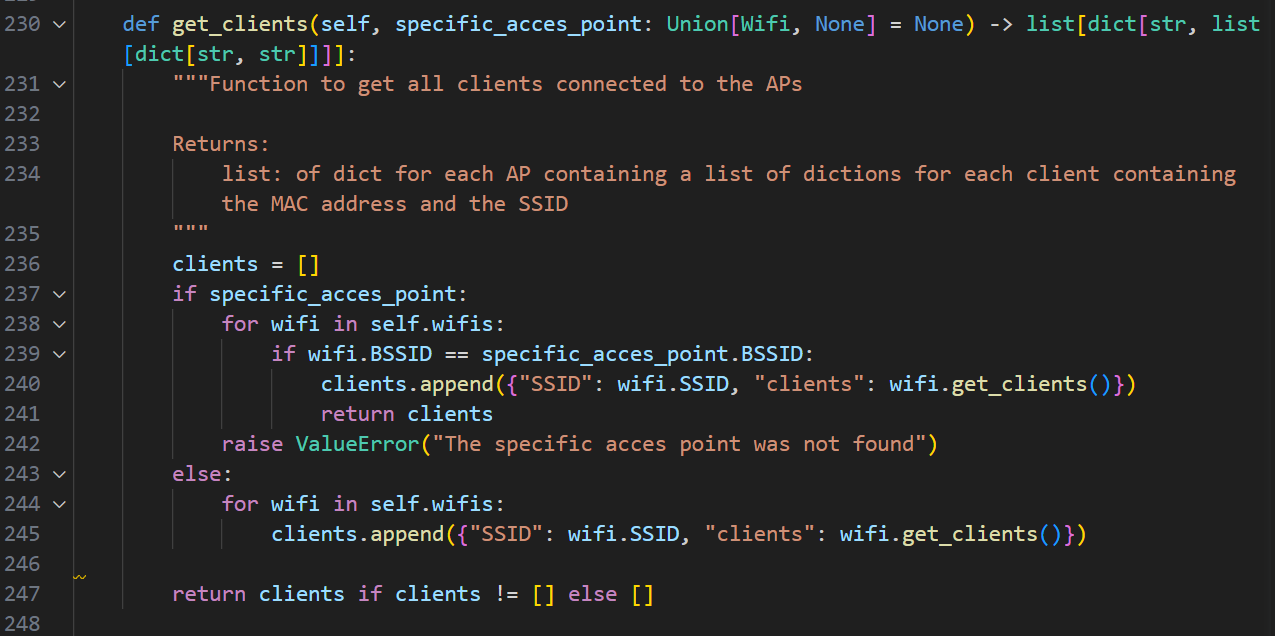
\includegraphics[width=0.45\textwidth]{Latex-Files/Billeder/Implementation/Get_Clients.png}
    \caption{Code for getting the clients for each AP}
    \label{Scan2}
\end{figure}

When scanning for clients all 802.11 packets are examined as it is rare that there is communication between APs. However the DS fields in the 802.11 header is exploited, as they indicate the direction of the frame. The code for this is seen on figure \ref{Scan3}. 

\begin{figure}[!htbp]
    \centering
    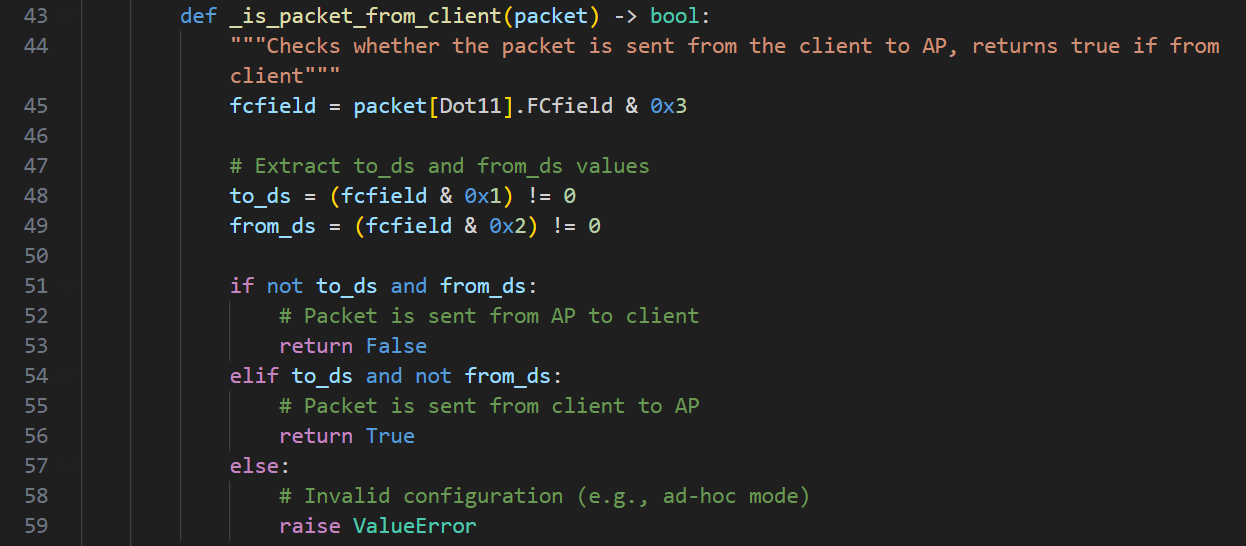
\includegraphics[width=0.5\textwidth]{Latex-Files/Billeder/Implementation/DS.png}
    \caption{Code for examining packets DS field}
    \label{Scan3}
\end{figure}


\begin{figure}[!htbp]
    \centering
    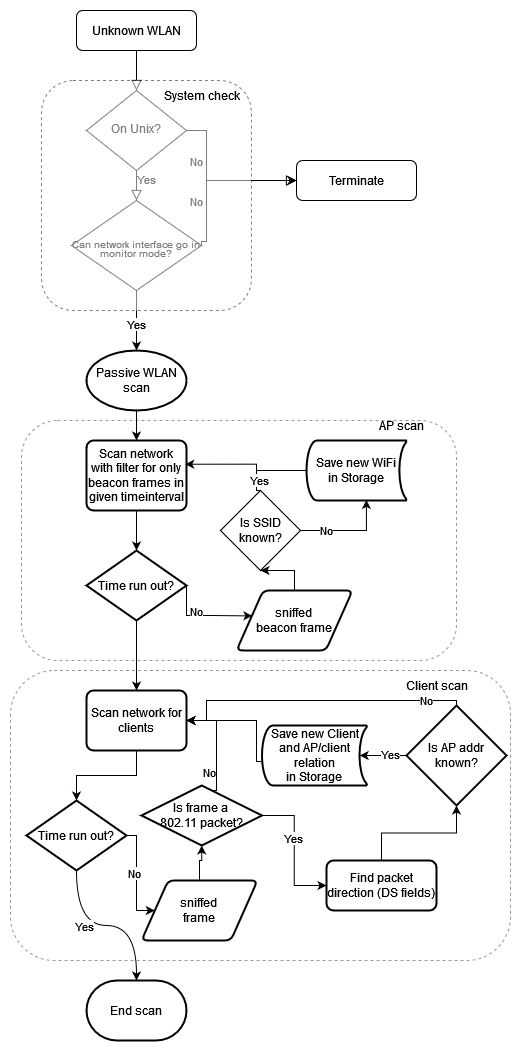
\includegraphics[width=0.5\textwidth]{Latex-Files/Billeder/Flowcharts/network_flowchart.png}
    \caption{Flowchart for mapping of WLAN}
    \label{Flowchart}
\end{figure}

Further optimization can be done to create better filters and most importantly use all data sent over the medium to create a more complete map of the WLAN. This however has not been done in the current level of implementation and might be deemed unnecessary as the wanted data is obtained.

\subsubsection{Limitations}
The implementation is limited to only being able to scan for APs and clients in the 2.4 GHz band. This is a physical limitation due to the fact that the dongle used for the implementation only supports the 2.4 GHz band.
The mapping of the network is done by passively scanning the medium, thus resulting to the implementation being limited to only having the ability to scan for APs and clients that are actively sending data. This is a limitation that is inherent to passive scanning. This can be overcome by using active scanning e.g. via a Replay Attack (which can force a device to send packets).
When doing the deauthentication attack there is actually a form of active scanning as the system is sending packets to the AP. This is however not a reliable way of scanning for APs and clients, as the current implementation of the attack is not built for this purpose and rather builds upon the passive scanning.
But the limitation of using passive scanning is also one of its positives: Since there is no active participation in the communication, the implementation is close to impossible to be detected by a WIDS (WiFi Intrusion Detection System). This is a positive as it allows for the implementation to be used for reconnaissance without being detected, whereas active scanning is noisy. NMAP a known tool for mapping networks (on ethernet) is very noisy and easy to detect.


\subsection{Deauthentication}
Our implementation of the deauthentication functionality relies on the ability to create and send packets with the use of Scapy. Thereby forging our own deauthentication packet, thus gaining the ability to set our own parameters for the packet.
As shown in figure \ref{deauth_prompt_code}, our implementation of the deauthentication is as follows. 

The user is first met with a menu of the known APs, gained from the mapping of the network, that are eligible for attempting an attack.
We have then decided to show another prompt menu which gives the user the option of choosing the target from a list of the already known clients, if so desired. If not, the user can either input a MAC-address, or choose to use the broadcast address, resulting in all clients receiving the deauthentication packets. 

\begin{figure}[!htbp]
     \centering
     \begin{subfigure}{0.49\textwidth}
         \centering
         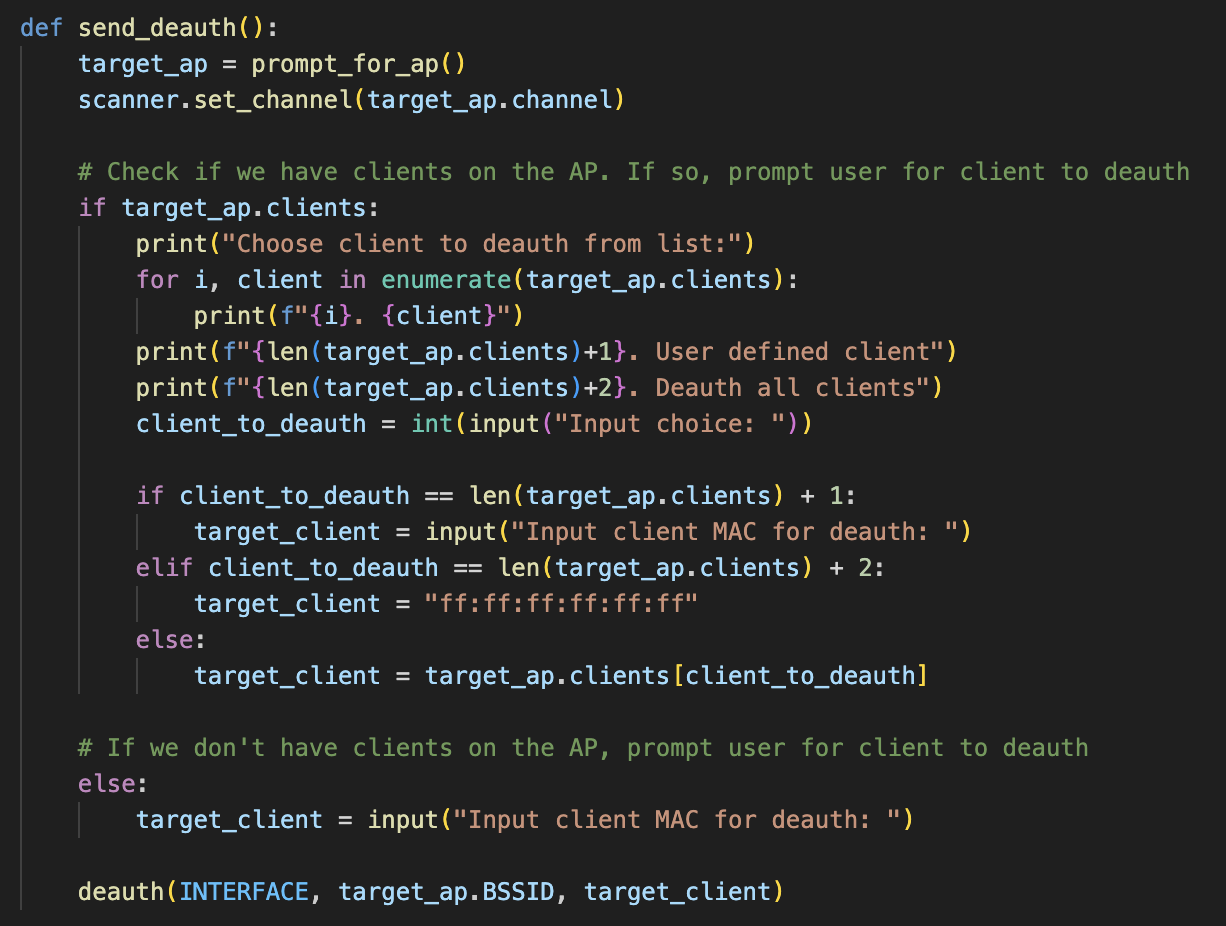
\includegraphics[width=\textwidth]{Latex-Files/Billeder/Implementation/deauth_prompt_code.png}
         \caption{Code for prompt and call of attack}
         \label{deauth_prompt_code}
     \end{subfigure}
     \hfill
     \begin{subfigure}{0.49\textwidth}
         \centering
         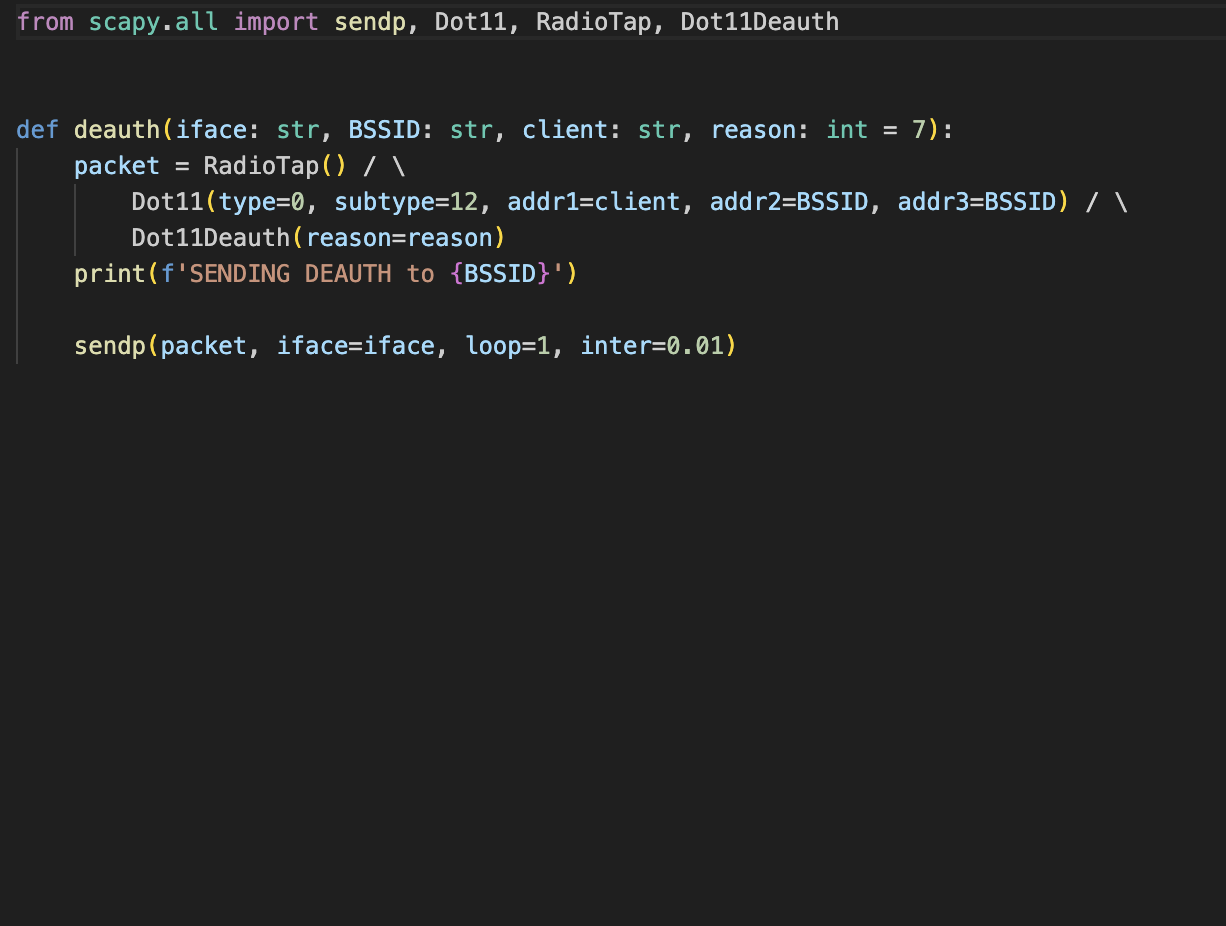
\includegraphics[width=\textwidth]{Latex-Files/Billeder/Implementation/deauth_func_code.png}
         \caption{Code for deauthentication attack function}
         \label{deauth_func_code}
     \end{subfigure}
     \hfill
     \caption{}
\end{figure}

After a target AP, and a target client has been defined, the "deauth" function, seen in figure \ref{deauth_func_code}, is then called. This function is what creates the appropriate deauthentication packets. The instantiation of the packet works by stacking layers on top of each other. In this case the packet is created by first making a RadioTap layer, which is responsible for sending the packet we create.

Then a Scapy "Dot11" layer is made, which represents a basic 802.11 frame. Here the type i set to 0, indicating a management frame, and the subtype to 12 indicating a deauthentication frame. From here the addresses are defined for the target of the frame. \\Finally the last layer is added, this being the "Dot11Deauth" layer which here defines a reasoncode for the deauthentication. This reasoncode is set to be 7 for default, which corresponds to the reason "Class 3 frame received from non-associated STA" \cite{Cisco_Deathentication_reasoncodes}. In a communications relation, the reasoncode provides important information about the cause of the deauthentication. However it is not an integral part of the deauthentication action itself, therefore the reasoncode is just given as a random number we have chosen.
Although it does not have a functional use, the reasoncode could in practice improve a deauthentication attack, by using appropriate reasoncodes, thus further concealing the fact that it is of malicious nature.

Subsequently a line is printed to the console notifying the user that a deauthentication attack will commence, combined with the target for the attack.
Ultimatly the "sendp" function, sends the beforehand created deauthentication frame.

\begin{figure}[!htbp]
     \centering
     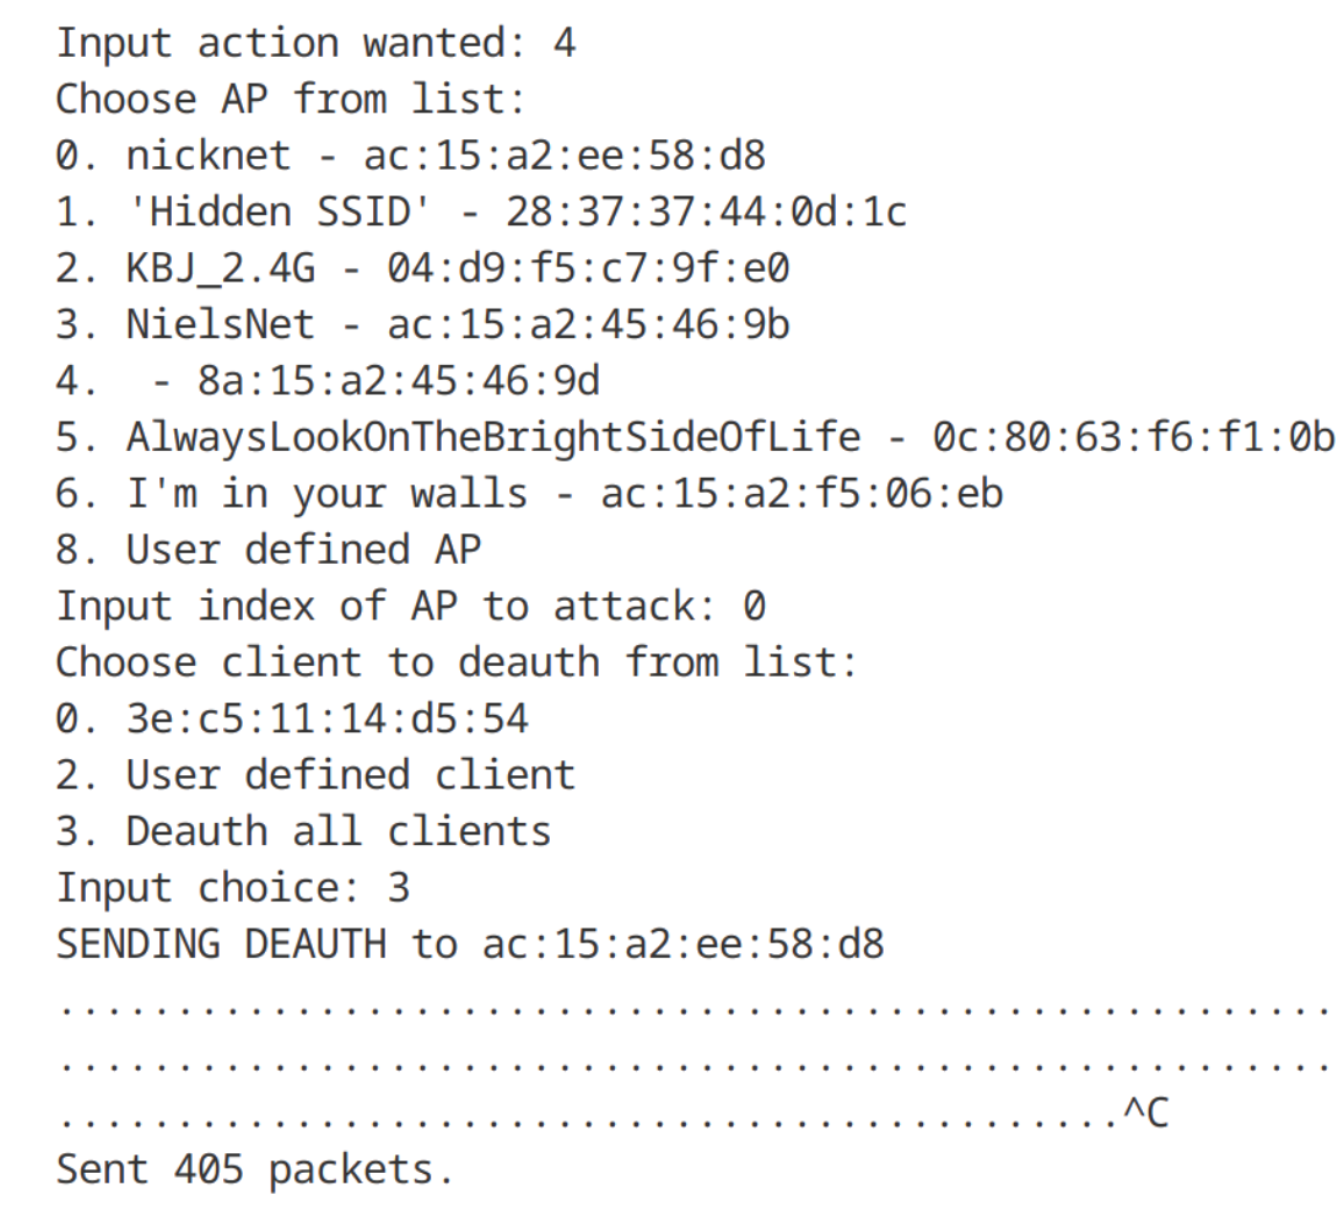
\includegraphics[width=0.7
     \textwidth]{Latex-Files/Billeder/Implementation/deauth_attack.png}
     \caption{Output when running deauthentication attack}
     \label{deauth_attack}
\end{figure}

Figure \ref{deauth_attack} shows the output presented to the user, when performing the deauthentication attack. The user can here choose to selectively deauthenticate a single client. Alternately the user possesses the option to deauthenticate all clients from the targeted AP. Upon the user inputting a choice, the program begins transmitting the packet constructed. The deauthentication attack is continuous and will only stop when interrupted by the user. 

Our deauthentication implementation has undergone limited testing, highlighting the need for further investigation. Our objective is to assess its functionality in various scenarios, including both successful and unsuccessful cases. Furthermore, we aim to evaluate the performance of the code by conducting tests on edge cases. Additionally, we plan to examine the behavior of the implementation when multiple clients are connected, observing whether all of them are successfully deauthenticated. 


\subsection{Password cracking}
The implementation of password cracking uses Scapy to read and save packets being sent on specific channels. It uses the implementation of the WiFi-scanner to get the APs that have the potential to be cracked. The function is as follows:

First a menu is shown where the user can chose between scanning for packets and cracking with the packets. If scanning is chosen, then he user is, like with deauthentication, shown a table of known APs. The user then choses which AP to crack. If an AP without WEP is chosen and error occurs. If not i begins to sniff packets on that AP's channel and saves every packet that contain a WEP part. This is done for a specific amount of time chosen by the user. 

Afterwards the packets are saved in a file that can then be read by Aircrack-ng if the other option on the menu is chosen. It runs Aircrack-ng in a console window and uses the saved file to crack the password. 

Aircrack-ng is made up of commands that is used to manipulate data, it it not code written directly. That has the consequence that most of the implementation will be in the mapping of networks part. 

The way Scapy saves the packets has the consequenses that Aircrack-ng cannot use the PTW method of cracking for passwords and subsequently it uses the lesser method which requires a minimum of 250.000 packets, about 15 times more packets. Therefore it needs a lot more time to crack the network. 


A succesful test has also been completed with the use of Airodump-ng which is a part of Aircrack-ng.
\newpage
\section{Tests}
We have tested our implementation.
\subsection{Mapping of networks}
We have done limited testing of our program. First we tested the mapping of networks as that is a requirement for the deauthentication. We tested on DTU campus which should give us APs that are connected to DTUsecure, eduroam, DTUdevice and DTUguest. It should also give us all clients nearby as their MAC address. The result is shown on figure \ref{test1}.

\begin{figure}[!htbp]
    \centering
    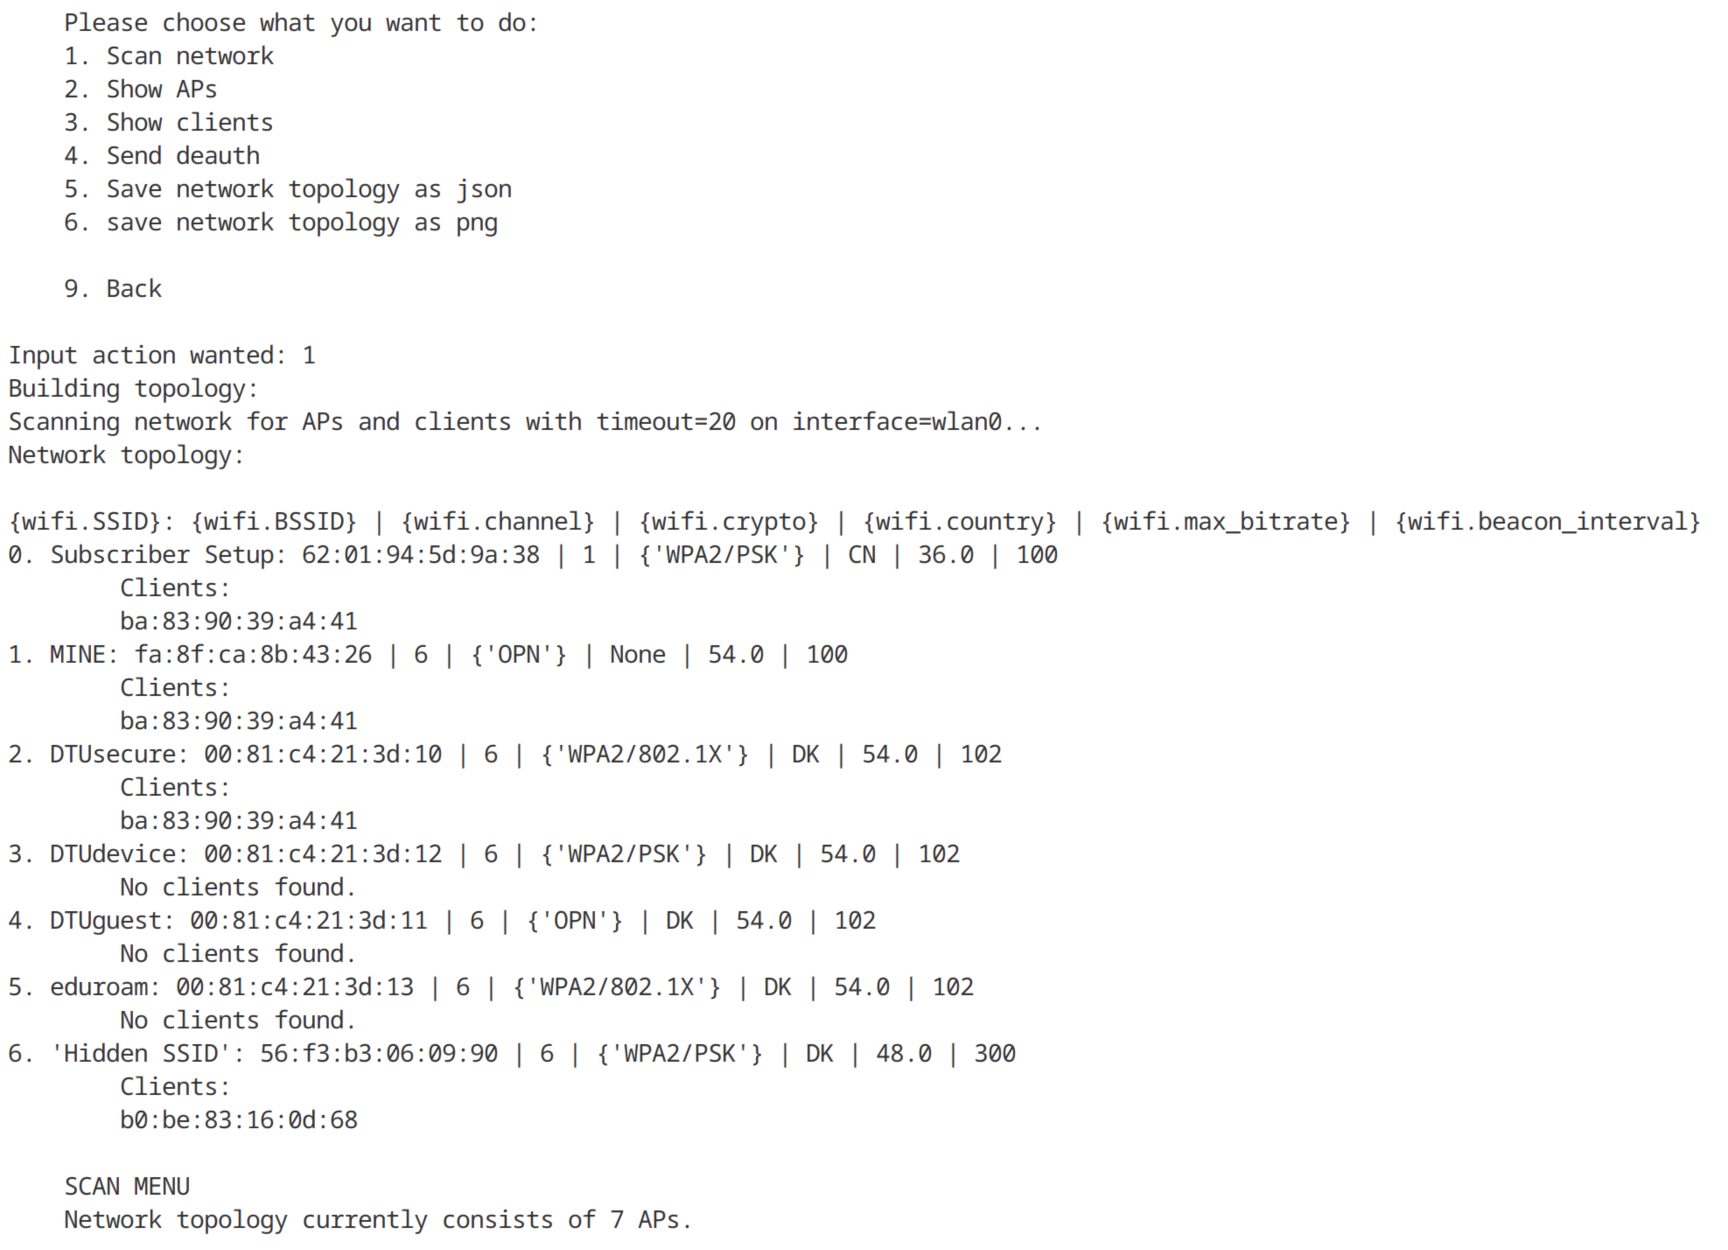
\includegraphics[width=\textwidth]{Latex-Files/Billeder/Tests/scan_network.png}
    \caption{Testing the network mapper}
    \label{test1}
\end{figure}

As we can see the test was successfully completed and DTUsecure, eduroam, DTUdevice and DTUguest showed up, together with some other APs unconnected to DTU. We have also found clients nearby. This shows that the mapping of networks has been successfully implemented in its simplest form. 

\subsection{Deauthentication}

Then we tested the deauthentication of a Macbook. It was connected to a smartphone set up as an AP and both the Macbook and the AP showed up. We started a constant ping on the Macbook and afterwards started the deauth attack. The pinging i shown on figure \ref{Test2}

\begin{figure}[!htbp]
     \centering
     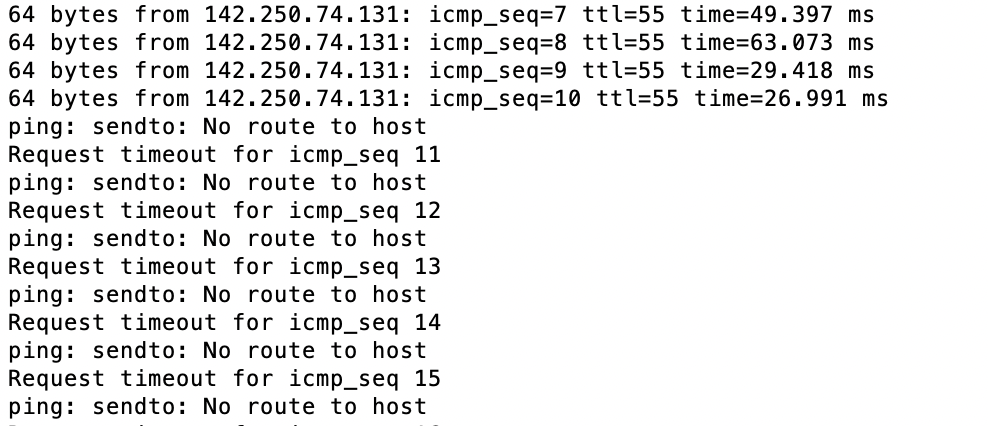
\includegraphics[width=0.5\textwidth]{Latex-Files/Billeder/Tests/deauth_ping.png}
     \caption{Result from being attacked (Mac)}
     \label{Test2}
\end{figure}

Figure \ref{Test2} shows the result of the attack. This attack was run by deauthenticating a single client. it is evident that the pinging to google works in absence of complications, however when the deauthentication attack is deployed, the pinging encounters issues and outputs "No route to host". Thereby denying the client service, and disconnecting the client from the internet. . We then tested on a Windows PC as seen on figure \ref{Test3}.

\begin{figure}[!htbp]
    \centering
    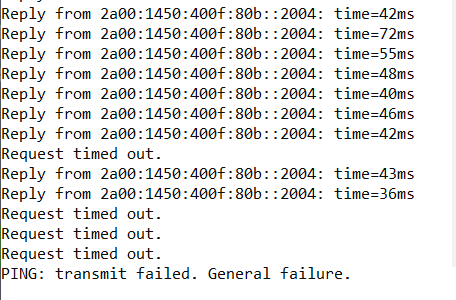
\includegraphics[width=0.5\textwidth]{Latex-Files/Billeder/Tests/Deauth virker.png}
    \caption{Result from being attacked (Windows)}
    \label{Test3}
\end{figure}

We can conclude that the deauthentication works on both Windows and MacOS. 

\begin{figure}[!htbp]
    \centering
    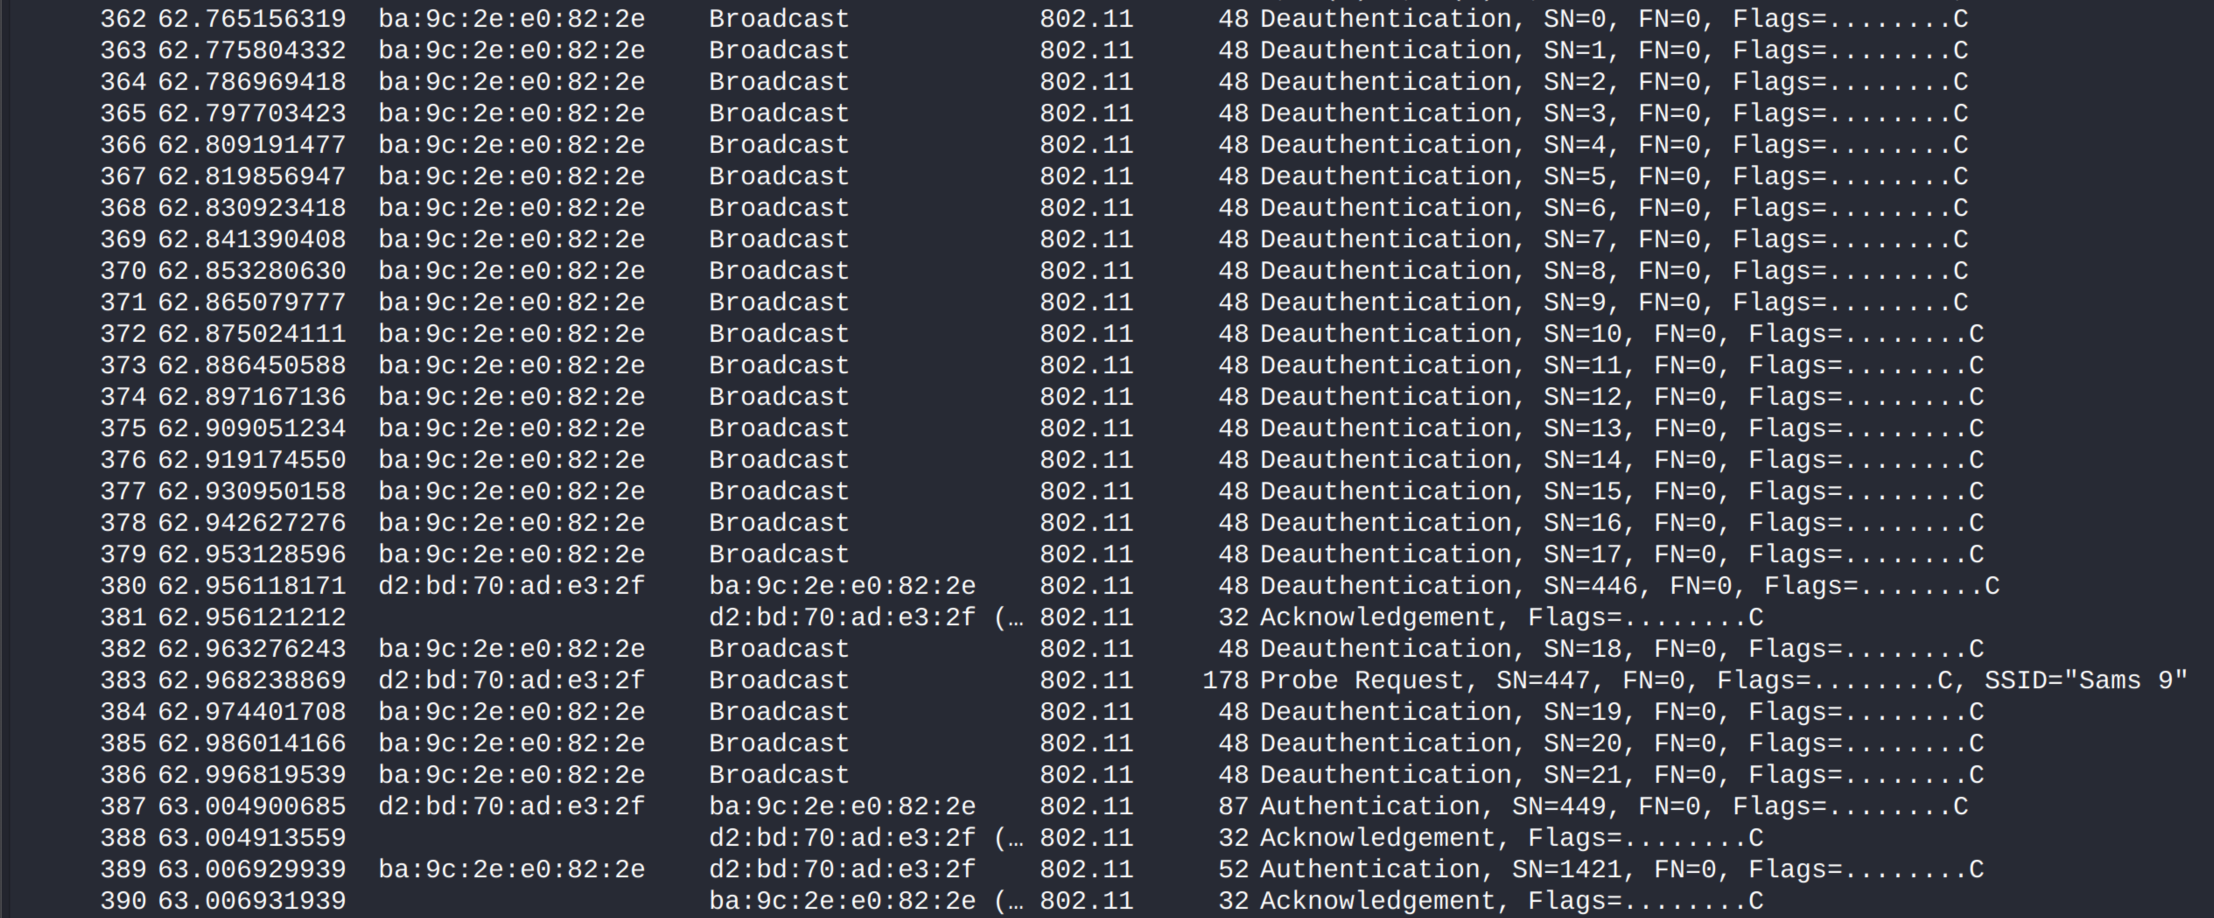
\includegraphics[width=0.7\textwidth]{Latex-Files/Billeder/Tests/deauth_pcap.png}
    \caption{pcap of deauthentication}
    \label{deauth_pcap}
\end{figure}

As well as testing the deauthentication by pinging, we have examined the packets themselves using wireshark. In figure \ref{deauth_pcap} the deauthentication packets sent out can be observed. It is evident that as expected, our program transmits deauthentication packets for the designated target. The deauthentication packets were, in this test, broadcasted in order to deauthenticate all clients connected to the AP. 
Notice packet number 381, which is an acknowledgement, thus confirming the deauthentication of the client.


\begin{figure}[!htbp]
    \centering
    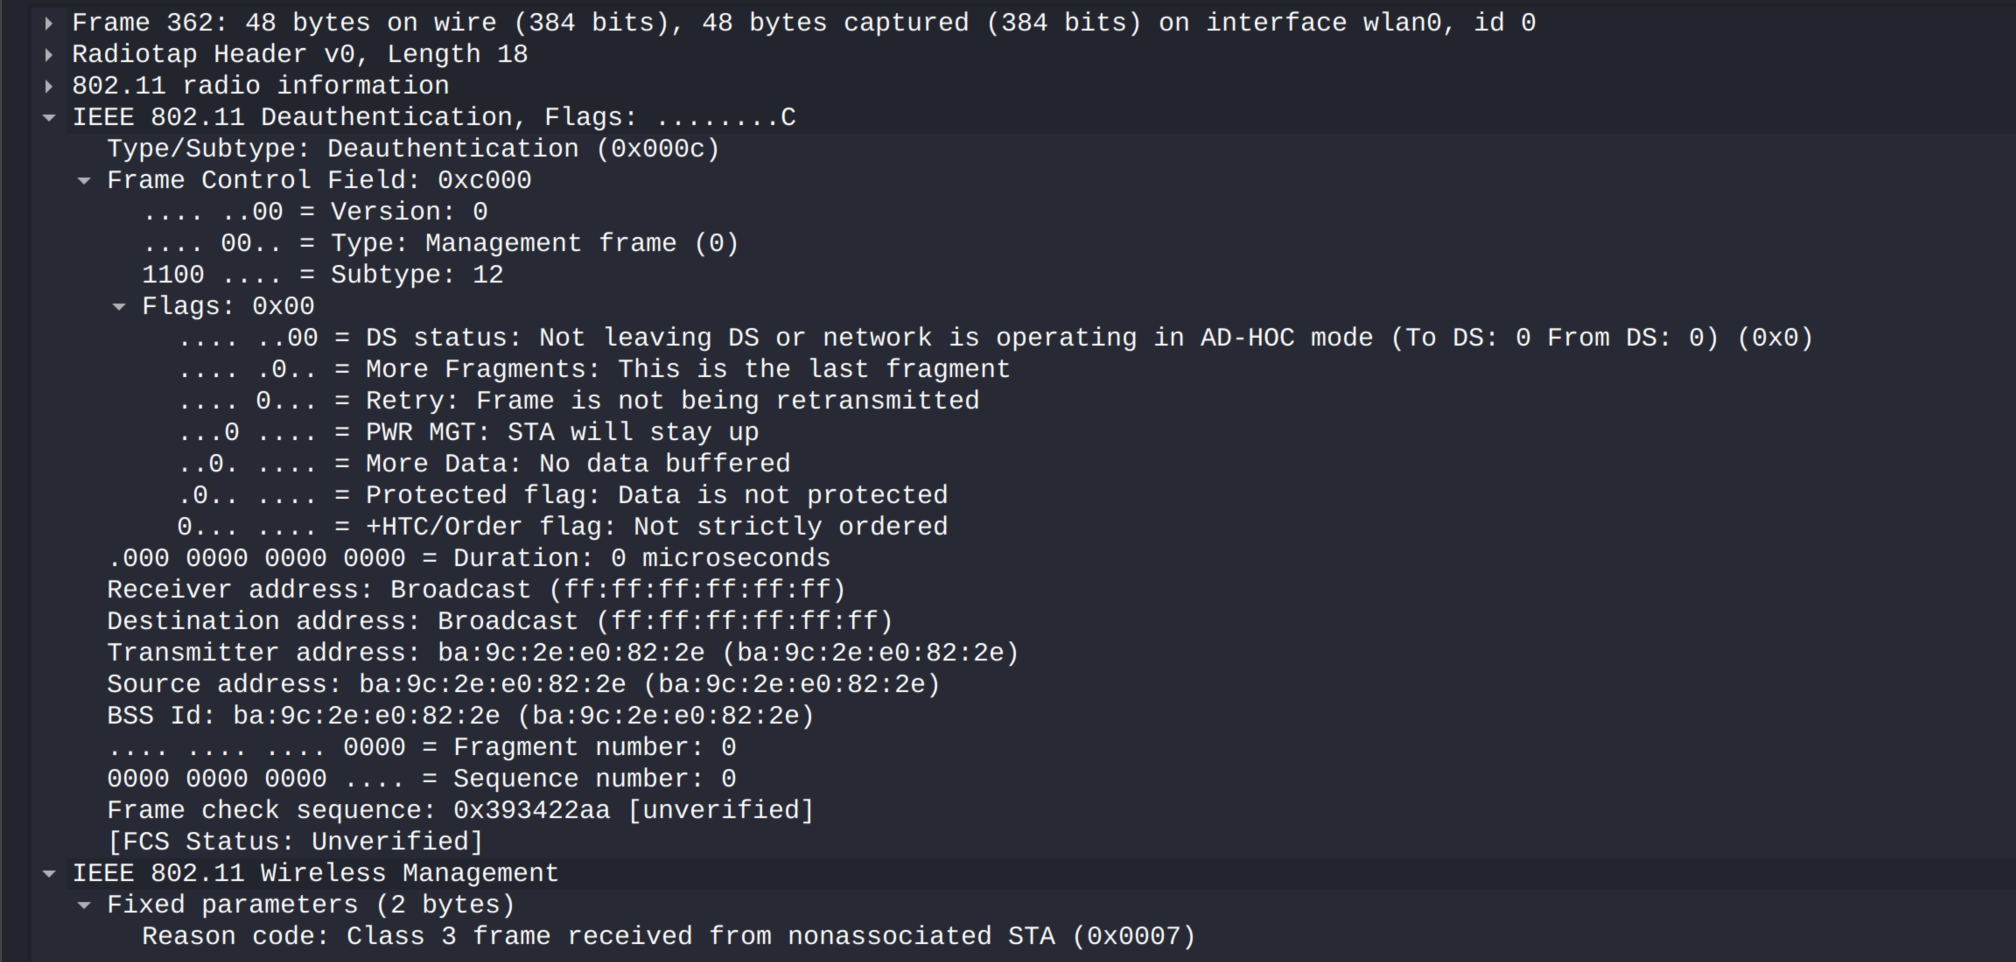
\includegraphics[width=0.7\textwidth]{Latex-Files/Billeder/Tests/deauth_pcap_packet.png}
    \caption{Deauthentication packet further inspection}
    \label{deauth_pcap_packet}
\end{figure}

Delving deeper into a particular deauthentication packet transmitted, as shown in figure \ref{deauth_pcap_packet}, we can observe the specific parameters set during the deauthentication. The reciever, and destination addresses are both set to the broadcast address, and the source address is set to the AP the clients will be disconnected from. Additionally the aforementioned reasoncode for the deauthentication.


\subsection{Password Cracking}
A test has been successfully done where, using Airodump-ng for capturing packets, a network has been cracked and the password found. 

\begin{figure}[!htbp]
    \centering
    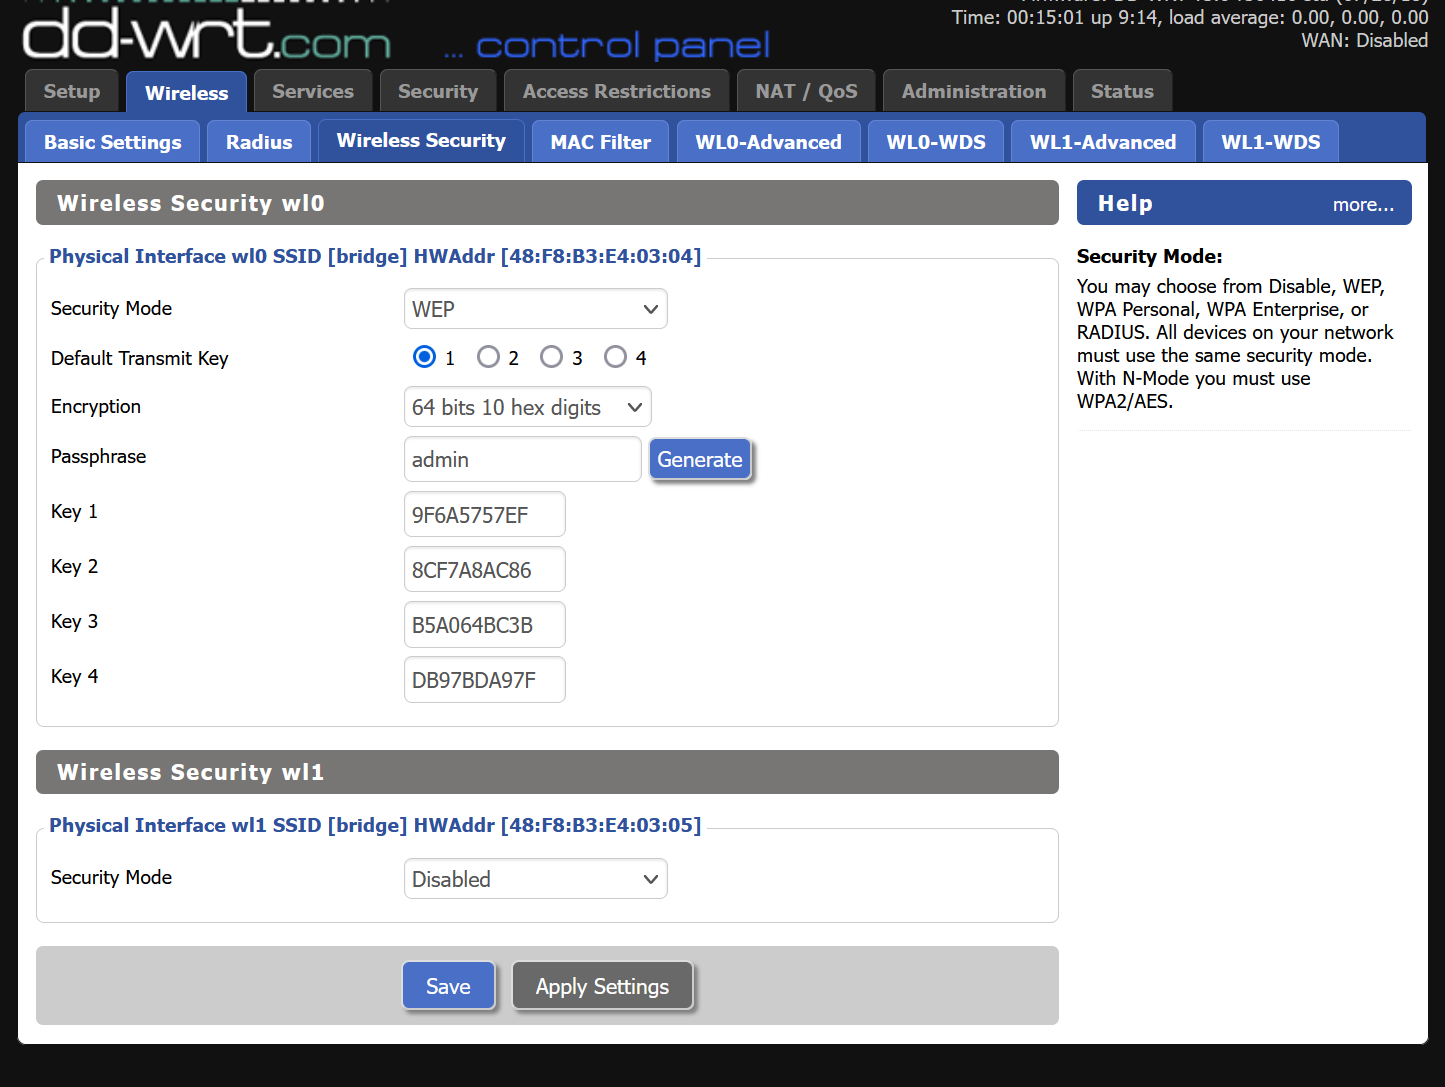
\includegraphics[width=0.5\textwidth]{Latex-Files/Billeder/Kode2.png}
    \caption{The passwords on the AP}
    \label{Crack2}
\end{figure}

The test was that an AP, with the capability to use WEP, was set up and connected to a wider network on the internet and then made to use WEP with passkeys, as seen on figure \ref{Crack2}. Then a computer using Linux was connected to that AP and a constant stream of data was created by watching YouTube. Then another computer was setup to monitor these data-packets and capture those that contain an initialization vector (IV). 

There was a small problem with the connection between the AP and the wider internet, so we had to constantly pull the ethernet plug and replug. This was probably because the wider network didn't like using WEP, and that was also why YouTube did not actually work. So the computer sent and received data-packets from the AP only. Enough data-packets where still created and so a large .pcap file was made with about 10.000 IV packets. 

\begin{figure}[!htbp]
    \centering
    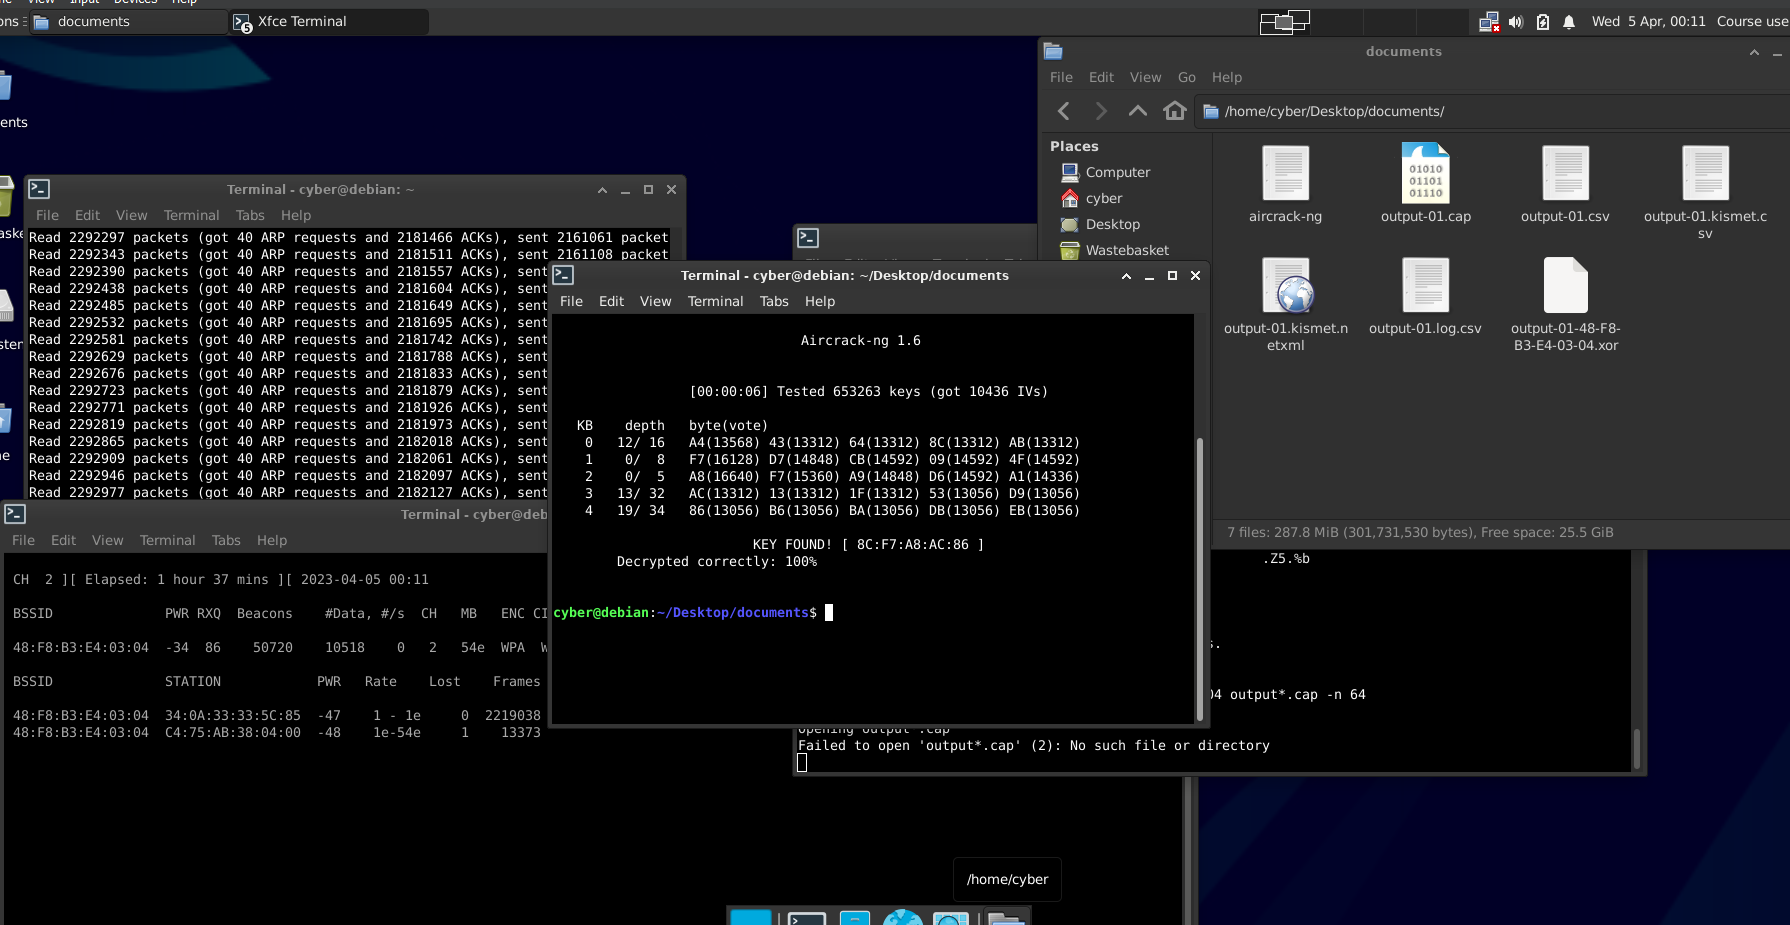
\includegraphics[width=0.8\textwidth]{Latex-Files/Billeder/Kode1.png}
    \caption{Aircrack-ng finding the password}
    \label{Crack1}
\end{figure}


Then Aircrack-ng was used on this .pcap file to find the passkey, which it did after 6 secounds. The passkey corresponds with one of the chosen passkeys on the AP. We can see the result on figure \ref{Crack1}.

Hopefully we can capture packets containing IV's using the WiFi-scanner and Scapy and place them in a combined file. That would make it simple to crack the WEP algorithm using Aircrack-ng and thereby recreating the passkeys and allowing access to the data-packets. 
\newpage
\section{Main Challenges}
Our main challenge in this project is the fact that internet traffic is complicated and made up of many interlocking parts. There is a lot of data being sent constantly and most of it is not relevant to what we are doing. As we are working with a shared medium it can be hard to differentiate between what we are creating and what is part of the standard traffic. That makes it difficult to figure out what is going on 'under the hood' when testing our implementations. Thus it has so far taken much longer to perform some of the basic steps of mapping the network and simple deauthentication. Still this is very much a learn by doing project in the way that we obtain solutions to either tackle or overcome the obstacles and after implementing our WiFi-scanner we have gained valuable knowledge about how data-packets are built. 

Likewise the theory behind most of the 802.11 management frames and such used in this project is very new to us, since only a short overview of 802.11 has been provided in our courses where the focus mainly has been on the EAPOL 4-way-handshake within WPA. Thus there is a great gap in knowledge we need to fill as some of the implementation parts require a deep understanding of how e.g. the procedure for deauthentication works.

When cracking WEP, the main challenge is figuring out how to create enough packets consistently that contain IV's and are use the same passkey. Also if this is successfully implemented we also have to recreate Aircrack-ng's PTW method to crack the WEP algorithm. Then this needs to be integrated with the rest of the code. 

The code that we have written is also hard to understand for outsiders, so we have to focus on rewriting the code to make it more understandable for everyone. It would also make expansion of features easier in the future. 
\newpage

\section{Discussion}

\section{Future Work}

\section{Conclusion}
In this project we have investigated network traffic by mapping local WiFi networks using python and the tool Scapy to show all APs connected and the clients connected to these networks. By obtaining knowledge of the WLAN it was managed to send deauthentication frames from a spoofed source address, hence doing a deauthentication attacks to disconnect one or more clients from using wireless networking. By doing this we gained advanced knowledge about different types of frames and subframes in the 802.11 standard as well as a thourough understanding of the attacks. The security algorithm in the 802.11, namely WEP has been examined and exploited to understand fundamental methods as statistical analyzis to exploit flaws in the algorithm. Yet there is still work left in order to explore mitigations for the different attacks. Likewise there is work left in order to ensure stability and integrity of the attacks, and anonymity when performing the attacks.  
During this project we also increased our knowledge of python programming and networking toolboxes that use python, which gives a broad understanding of how packets are structured. 



\section{Appendix}

\section{Peer Feedback}
We received feedback about some theory that should be added about Scapy. We fixed this by giving more information about Scapy.
We also changed how we inserted our code snippets as a screenshot of dark code makes it hard to read, so we fixed it by adding the code inside the report as text. 
We added a small section after the introduction showing who wrote what as it was proposed in the peer-review in order to obtain a quick overview.

\section{Reflections}
% whats learned process wise, ie the teamwork,timeplans, main working lessons learned

\section{Code}


